\section{Metodología}

Para el desarrollo del estudio, se adoptó el enfoque de Revisión Sistemática de la Literatura (RSL) con el propósito de recopilar, evaluar y sintetizar el material científico disponible acerca de las aplicaciones basadas en inteligencia artificial para la mejora de accesibilidad educativa en lenguas de bajos recursos. A su vez, se decidió usar la metodología PRISMA, una guía publicada en el año 2009 que marca un estándar de calidad para la elaboración de revisiones sistemáticas, garantizando transparencia, rigor y calidad de presentación. 
Asimismo, se empleó el marco de trabajo PICO (Población, Intervención, Comparación y Resultado) para delimitar con presición el alcance del estudio. Los componentes que integran este marco se definieron de la siguiente manera:

\begin{itemize}
   \item P: Estudiantes cuya lengua materna es una lengua de bajos recursos.
   \item I: Uso de herramientas basadas en Inteligencia Artificial (IA), grandes modelos de lenguaje (LLMs).
   \item C: Desempeño en lenguas de altos recursos.
   \item O: Mejora en la accesibilidad, personalización del aprendizaje, equidad educativa e innovación pedagógica.
\end{itemize}

A partir de esto, se formularon preguntas específicas que vinculen las lenguas de bajos recursos con Inteligencia Artificial (IA). Las preguntas formuladas se detallan en la tabla 1:


\begin{table}[H]
\centering
\captionof{table}{Estructura PICO}
\small
    \begin{tabular}{cp{4.6cm}}
    \toprule
    \multicolumn{1}{c}{\textbf{Esquema PICO}} & \multicolumn{1}{c}{\textbf{Preguntas}} \\
    \midrule
    P & ¿De qué manera las tecnologías de Procesamiento de Lenguaje Natural (NLP) benefician la integración de la lengua materna en entornos educativos? \\ \addlinespace
    I & ¿De qué manera las herramientas basadas en IA y LLMs mejoran la accesibilidad educativa? \\ \addlinespace
    C & ¿Qué vacíos existen entre el desempeño de la IA en lenguas de alto recurso frente a las de bajos recursos? 
 \\ \addlinespace
    O & ¿Qué estrategias y metodologías son las más eficaces para mejorar la accesibilidad educativa?
 \\
    \bottomrule
    \end{tabular}%
  \label{tabla1}%
\end{table}

De igual forma, la estrategia de búsqueda elaborada se basó en artículos procedentes únicamente de la base de datos Scopus, una de las bases de datos más prestigiosas a nivel mundial. Para la selección de artículos, se establecieron los siguientes criterios:

\begin{itemize}
   \setlength{\itemsep}{0pt}
   \setlength{\parskip}{0pt}
   \item Criterio 1 (C1): Estudios realizados en estudiantes cuya lengua nativa es de de bajos recursos.
   \item Criterio 2 (C2): Estudios que empleen IA, LLMs o Natural Language Processing (NLP).
   \item Criterio 3 (C3): Desempeño de herramientas basadas en IA en lenguas de altos recursos.
   \item Criterio 4 (C4): Estudios cuyo propósito sea mejorar la accesibilidad, mejorar el aprendizaje o promover la equidad educativa y pedagógica.
   \item Criterio 5 (C5): Estudios de áreas relacionadas a Ciencias de la Computación, Artes y Humanidades, Ciencias Sociales, Ingeniería y Matemáticas.
\end{itemize}

Asimismo, la tabla 2 detalla la metodología empleada para la búsqueda: se presenta la pregunta de investigación formulada en base a las preguntas del esquema PICO, palabras clave identificadas, ecuación general de búsqueda y los criterios de selección empleados, más adelante siendo usados en la exclusión de artículos.


\begin{table}[H]
\centering
\captionof{table}{Metodología usada para la búsqueda}
\small
\begin{tabular}{|p{2cm}|p{5.3cm}|}
\hline
\centering{Parámetros de búsqueda} 
& \centering\arraybackslash{Parámetros de búsqueda de la información} \\
\hline

{Pregunta de investigación} 
& ¿De qué manera la integración de la Inteligencia Artificial impacta en la accesibilidad educativa y la calidad de la información recuperada por estudiantes de lenguas de bajos recursos, en comparación con lenguas de altos recursos? \\
\hline

{Palabras clave} 
& Low-resource languages, minority languages, linguistic barriers, Artificial intelligence, large language models, natural language processing, high-resource languages, thematic dispersion,  Educational accessibility, educational equity, personalized learning, pedagogy. \\
\hline

{Base de datos} 
& Scopus. \\
\hline

{Intervalo de fechas} 
& 2022--2026. \\
\hline

{Ecuación general de búsqueda} 
& 
("Artificial Intelligence" OR AI OR "Large Language Models" OR LLM* OR "Natural Language Processing" OR "NLP" OR "Machine Learning" OR "Generative AI" OR "Machine Translation" OR "Language Technolog*")
AND
("low-resource language*" OR "under-resourced language*" "minority language*" OR "indigenous language*" OR "linguistic barrier*" OR "endangered language*" OR "language barrier*" OR Quechua OR Aymara)
AND
("educational accessibility" OR "educational equity" OR "personalized learning" OR education* Or teach* Or learn* OR pedagog*) \\
\hline

{Idioma}
&
Inglés. \\
\hline

{Tipo de documento}
&
Artículo, conference paper, revisiones. \\
\hline

{Accesibilidad}
&
Open access. \\
\hline

{Criterios de selección}
&
Estudios que aborden el uso de inteligencia artificial en el procesamiento, enseñanza o accesibilidad de lenguas de bajos recursos o lenguas de altos recursos.  \\
\hline

\end{tabular}
\label{tabla:parametros_busqueda}
\end{table}

La búsqueda en Scopus identificó 118 artículos, de los cuales 87 fueron excluidos debido a su antigüedad, falta de acceso abierto o ser capítulos de libros. De los 31 restantes, 4 no cumplieron con el criterio 5 de inclusión. Finalmente, pudo recuperarse un total de 27 artículos. La figura 1 muestra el diagrama PRISMA que detalla el proceso completo (identificación, evaluación y selección).

\begin{figure}[H]
\begin{center}
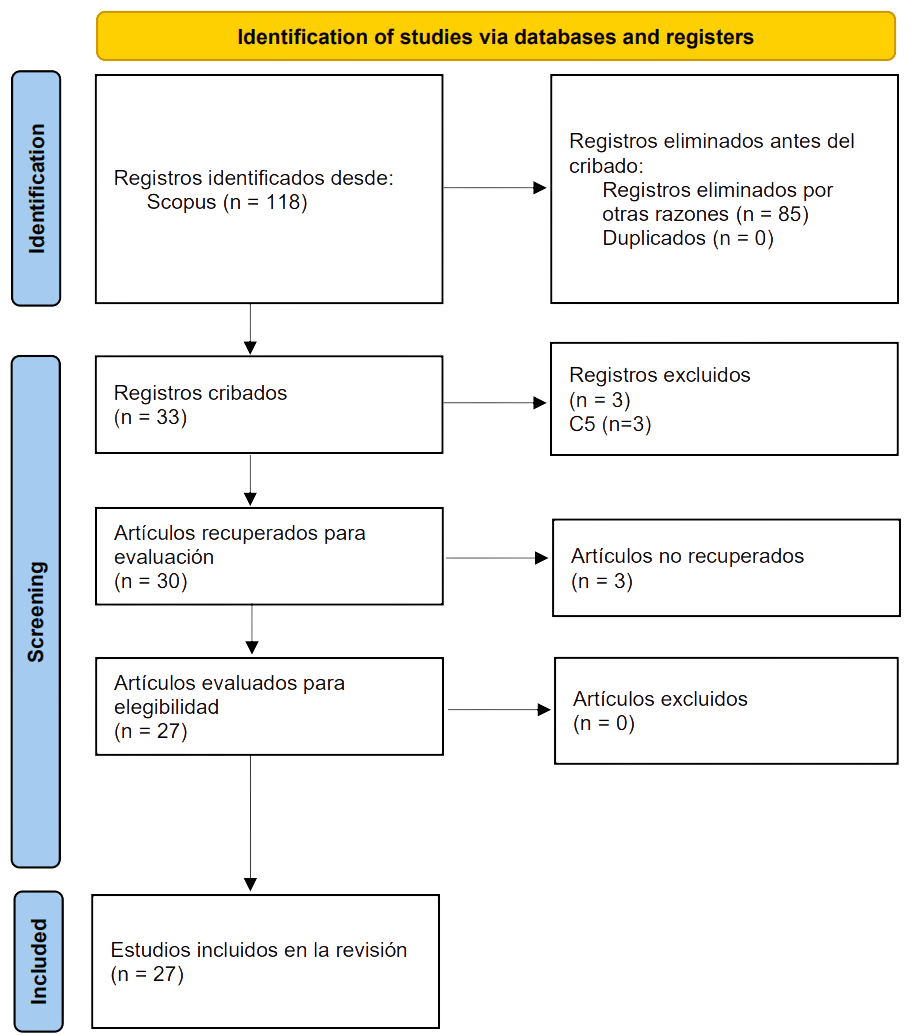
\includegraphics[width=7.8cm]{figures/fig1.png}
\end{center}
\caption{Diagrama de Prisma}
\label{figura1}
\end{figure}


% Las secciones de Introducción, Materiales y Métodos, Resultados y Discusión y Conclusiones del artículo pueden estructurarse divididas en diferente forma. En cada epígrafe del artículo se deben enumerar como máximo hasta tres niveles: 1. / 1.1. / 1.1.1. En esta plantilla en la sección materiales y métodos se explica cada una de las partes del manuscrito y como elaborarlo.

% \subsection{Título principal}

% El título principal (en la primera página) debe estar centrado, se debe respetar el codigo establecido para el efecto, respetando además el orden de mayusculas y minusculas, ya que el mismo se mostrará después de la compilación con la tipografía de fuente \textsc{Versalitas}.

% \subsection{Nombre del Autor(s) y afiliaciones}

% Los nombres del autor(es) deben estar centrados abajo del título y deben ser ingresados en el código indicado, tal como se indica en la parte superior de este documento.
%       Se escribirá primero el nombre y luego el apellido. En el caso de que el artículo tenga más de un autor, los nombres estarán separados por comas de manera que todos los nombres se los autores estén en una sola línea. Los detalles de los autores no deben mostrar ningún título profesional como PhD, MSc, Dr.

% \subsection{Títulos de primer, segundo y tercer nivel}

% El primer nivel corresponde al título principal de cada epígrafe, use el comando "\emph{section}", se debe usar un punto después del número del título.

% El segundo nivel corresponde a los subtitulos use el comando "\emph{subsection}"; mientras que para los subtitulos de tercer nivel use el comando "\emph{subsubsection}" 

% La configuración de esta plantilla permitirá que en cada nivel se muestre el tamaño de texto que identifique a cada uno.

% \subsection{Texto principal}

% El texto principal del artículo deberá ser colocado respetando las reglas gramaticales la condiguración de la plantilla mostrará los espaciados, tipo de fuente, sangrías, etc.

% \subsection{Figuras, tablas, ecuaciones, unidades y abreviaturas.}

% Figuras: Todas las figuras deben estar cargadas en la carpeta del código fuente denominada "\emph{figures}" con un nombre caracteristico que identifique a cada figura que conste en el artículo, utilice el código a continuación indicado para llamar a cada figura según corresponda en el texto del artículo, de la misma manera en el campo "\emph{caption}" colocar el nombre de la figura. Las figuras pueden estar en formato .jpg .png o .pdf con una resolución mínima de 300 dpi (ver Figura \ref{figura1}). También se pueden insertar código para figuras que usen el paquete TiKz o Pgfplots como muestra la Figura \ref{figura2}. Todas las figuras deben estar citadas en el texto. Si la figura posee dos partes incluya los indicativos “(a)” y “(b)” 

% \begin{figure}[H]
% \begin{center}
% 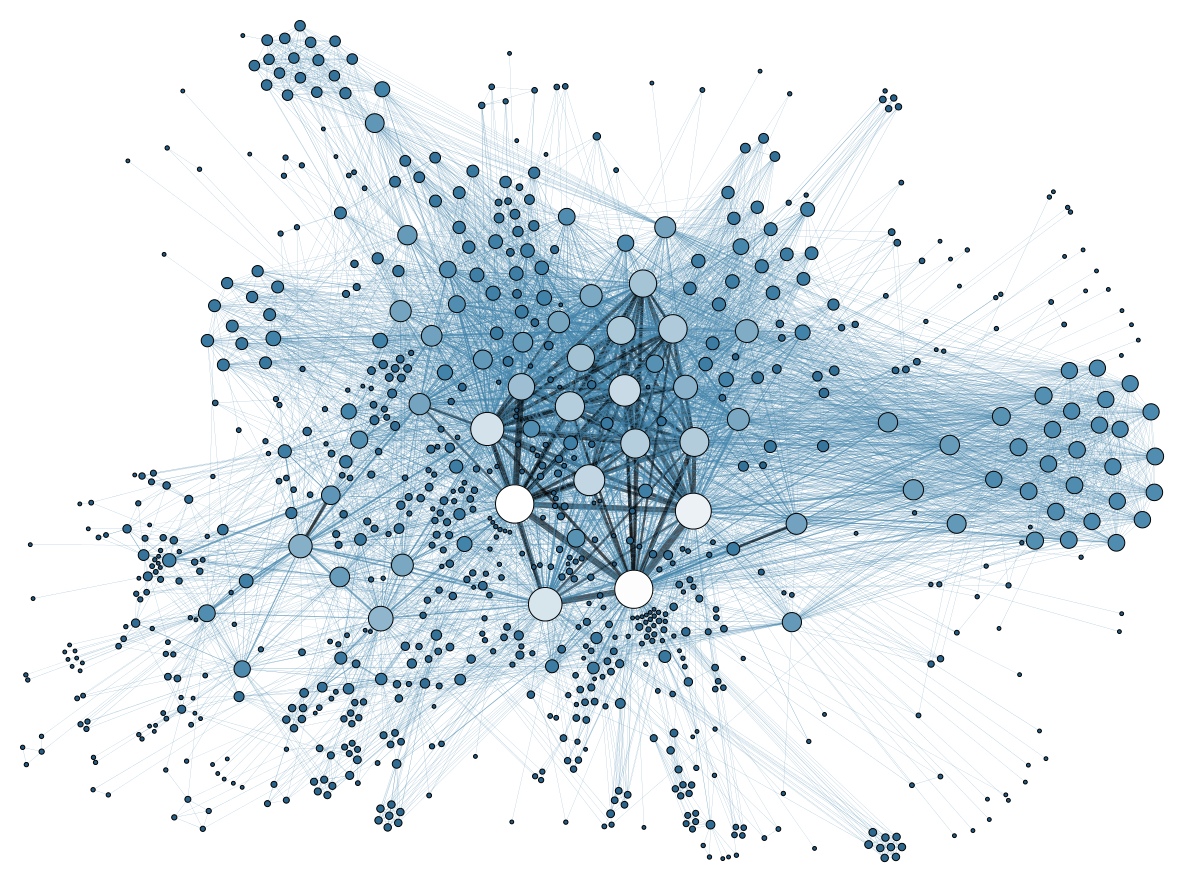
\includegraphics[width=7.8cm]{figures/fig2.png}
% \end{center}
% \caption{Nombre de la Figura.\cite{Mahmood2015}}
% \label{figura1}
% \end{figure}

% \begin{figure}[H]
% \centering
% %\label{fig2}
% \resizebox{6cm}{!} {
% \begin{tikzpicture}%
%    \begin{axis}[
%       ylabel style={overlay},
%       yticklabel style={overlay},
%       xlabel={$x$},
%       ylabel={$y$},
%       legend style={at={(0.5,0.97)},
%          anchor=north,legend columns=-1},
%       domain=-2:2
%    ]
%    \addplot {x^2};
%    \addplot {x^3};
%    \addplot {x^4};
%    \legend{$x^2$,$x^3$,$x^4$}
%    \end{axis}
% \end{tikzpicture}
% }
% \caption{El título}
% \label{figura2}
% \end{figure}

% Tablas: Coloque las tablas al inicio o al final de las columnas. A diferencia de las figuras el título de las tablas se coloca en la parte superior de la misma. 
% En la Tabla \ref{tabla1} de esta guía se muestra un ejemplo del formato para la presentación del artículo.
% Debe verificar que igual que las figuras, las tablas que se encuentren en el artículo se citen en el texto principal. 

% \begin{table}[H]
% \centering
% \captionof{table}{Tamaños de Fuente que se utilizan en la plantilla de articulos de la revista INGENIUS}
%   \scalebox{0.74}{
%     \begin{tabular}{cl}
%     \toprule
%     \multicolumn{1}{c}{Tamaño de letra} & \multicolumn{1}{c}{Uso} \\
%     \midrule
%     \small{10}    & \small{Datos del autor, título, texto de tablas y figuras.} \\
%     {\textbf{12}} & \textbf{Resumen, palabras clave} \\
%     12    & Nombre del autor(es), texto del artículo  \\
%     \Large{13}    & \Large{Títulos de segundo y tercer orden} \\
%     \LARGE{\textbf{15}} & \LARGE{\textbf{Títulos de primer nivel}} \\
%     \huge{\textbf{18}} & \huge{\textbf{TITULO}} \\
%     \bottomrule
%     \end{tabular}%
% }
%   \label{tabla1}%
% \end{table}

% Ecuaciones: Utilice editor de ecuaciones desde OverLeaf.  Trate de que las ecuaciones sean compactas empleando en el signo (/), la función exponencial como exp, o subíndices y superíndices. Las ecuaciones requeridas dentro del modelo matemáticas serán enumeradas según se detalla a continuación en la Ec \ref{eq1}.

% \begin{equation} 
% \label{eq1}
% \begin{array}{ll}
% \alpha = \frac{l + s}{s} * \lambda & [veh]
% \end{array}
% \end{equation}

% Unidades: Las unidades recomendadas son las del sistema métrico, en particular, se sugiere el uso del Sistema Internacional de Unidades (Unidades SI). Las unidades del sistema inglés pueden emplearse como unidades secundarias (en paréntesis). 

% Abreviaturas: Se deben definir las abreviaturas y acrónimos que no sean comunes la primera vez que aparecen en el texto, aún si ya se han definido en el resumen. No utilice abreviaturas en el título a menos que sea inevitable.

% \subsection{Referencias}

% Se debe verificar con cuidado que todas las citas colocadas en el texto, aparezcan en la lista de referencias bibliográficas. En la lista solo deben aparecer las referencias que fueron utilizadas en el texto principal del trabajo, en las tablas o en las figuras, esto implica que no deben aparecer otras referencias aunque el autor las haya consultado durante la preparación del artículo.

%         Las referencias incluidas en el texto se presentan al final ordenadas numéricamente en paréntesis cuadrados \cite{Valenzuela2019} según el orden de aparición en el texto. Un punto debe seguir al paréntesis \cite{Panwar2019}. Referencias múltiples pueden citarse con paréntesis separados por un guión \cite{Ramirez2015,Pagani2014,Peralta2017}. Cuando se cite un libro indicar las páginas con la información relevante. El título como tal de las “Referencias” al final del artículo no va numerado.
        
% Puede consultar la guía del IEEE para la cita de referencias disponible en el link: \url{https://bit.ly/2PjrnJj}

% Las referencias deben ser guardadas en el archivo \textbf{referencias.bib} en formato bibtex, indicando la \textbf{bibkey} secuencialmente según su aparición. Se recomienda utilizar un gestor bibliográfico para que pueda corregir previamente los metadatos como: autor, título, publisher, volume, issue, año, páginas, en caso de ser incorrectos \textbf{Mendeley}
